% !TeX program = xelatex
\documentclass{article}
\usepackage{svg}
\usepackage{amsmath}
\usepackage{amsfonts}
\usepackage{longtable}
\usepackage{booktabs}
\usepackage{hyperref}
\usepackage{mdframed}
\providecommand{\tightlist}{%
  \setlength{\itemsep}{0pt}\setlength{\parskip}{0pt}}
\usepackage{color}
\usepackage{fancyvrb}
\newcommand{\VerbBar}{|}
\newcommand{\VERB}{\Verb[commandchars=\\\{\}]}
\DefineVerbatimEnvironment{Highlighting}{Verbatim}{commandchars=\\\{\}}
% Add ',fontsize=\small' for more characters per line
\usepackage{framed}
\definecolor{shadecolor}{RGB}{248,248,248}
\newenvironment{Shaded}{\begin{snugshade}}{\end{snugshade}}
\newcommand{\KeywordTok}[1]{\textcolor[rgb]{0.13,0.29,0.53}{\textbf{#1}}}
\newcommand{\DataTypeTok}[1]{\textcolor[rgb]{0.13,0.29,0.53}{#1}}
\newcommand{\DecValTok}[1]{\textcolor[rgb]{0.00,0.00,0.81}{#1}}
\newcommand{\BaseNTok}[1]{\textcolor[rgb]{0.00,0.00,0.81}{#1}}
\newcommand{\FloatTok}[1]{\textcolor[rgb]{0.00,0.00,0.81}{#1}}
\newcommand{\ConstantTok}[1]{\textcolor[rgb]{0.00,0.00,0.00}{#1}}
\newcommand{\CharTok}[1]{\textcolor[rgb]{0.31,0.60,0.02}{#1}}
\newcommand{\SpecialCharTok}[1]{\textcolor[rgb]{0.00,0.00,0.00}{#1}}
\newcommand{\StringTok}[1]{\textcolor[rgb]{0.31,0.60,0.02}{#1}}
\newcommand{\VerbatimStringTok}[1]{\textcolor[rgb]{0.31,0.60,0.02}{#1}}
\newcommand{\SpecialStringTok}[1]{\textcolor[rgb]{0.31,0.60,0.02}{#1}}
\newcommand{\ImportTok}[1]{#1}
\newcommand{\CommentTok}[1]{\textcolor[rgb]{0.56,0.35,0.01}{\textit{#1}}}
\newcommand{\DocumentationTok}[1]{\textcolor[rgb]{0.56,0.35,0.01}{\textbf{\textit{#1}}}}
\newcommand{\AnnotationTok}[1]{\textcolor[rgb]{0.56,0.35,0.01}{\textbf{\textit{#1}}}}
\newcommand{\CommentVarTok}[1]{\textcolor[rgb]{0.56,0.35,0.01}{\textbf{\textit{#1}}}}
\newcommand{\OtherTok}[1]{\textcolor[rgb]{0.56,0.35,0.01}{#1}}
\newcommand{\FunctionTok}[1]{\textcolor[rgb]{0.00,0.00,0.00}{#1}}
\newcommand{\VariableTok}[1]{\textcolor[rgb]{0.00,0.00,0.00}{#1}}
\newcommand{\ControlFlowTok}[1]{\textcolor[rgb]{0.13,0.29,0.53}{\textbf{#1}}}
\newcommand{\OperatorTok}[1]{\textcolor[rgb]{0.81,0.36,0.00}{\textbf{#1}}}
\newcommand{\BuiltInTok}[1]{#1}
\newcommand{\ExtensionTok}[1]{#1}
\newcommand{\PreprocessorTok}[1]{\textcolor[rgb]{0.56,0.35,0.01}{\textit{#1}}}
\newcommand{\AttributeTok}[1]{\textcolor[rgb]{0.77,0.63,0.00}{#1}}
\newcommand{\RegionMarkerTok}[1]{#1}
\newcommand{\InformationTok}[1]{\textcolor[rgb]{0.56,0.35,0.01}{\textbf{\textit{#1}}}}
\newcommand{\WarningTok}[1]{\textcolor[rgb]{0.56,0.35,0.01}{\textbf{\textit{#1}}}}
\newcommand{\AlertTok}[1]{\textcolor[rgb]{0.94,0.16,0.16}{#1}}
\newcommand{\ErrorTok}[1]{\textcolor[rgb]{0.64,0.00,0.00}{\textbf{#1}}}
\newcommand{\NormalTok}[1]{#1}

\title{Teoría de la Información\\Solucionario}
\date{Curso 2023 - 2024}
\author{Lucas Goiriz Beltrán\\ Instituto de Biología Integrativa de Sistemas\\(I$_2$SysBio; UV-CSIC)\\Departamento de Matemática Aplicada\\Universitat Politècnica de València (UPV)}

\begin{document}
\maketitle

\section{Ejercicios de Entropía y Fuentes de Información}

\textbf{
1. Sea $X$ una variable aleatoria que toma valores sobre un alfabeto $\mathcal{A} = \left\{x_1,x_2,x_3,x_4,x_5\right\}$ con las correspondientes probabilidades $P = \left\{0.1,0.2,0.3,0.05,0.35\right\}$. Calcula la entropía de $X$ y compárala con la de una variable aleatoria que tome valores sobre el mismo alfabeto, pero con una distribución uniforme.
}

\vspace{0.5cm}

Calculamos la entropía de $X$ como:

\begin{align*}
    H(X) &= -\sum_{i=1}^{5}P(x_i)\log\left(P(x_i)\right)\\
    &= -0.1\log (0.1) - 0.2\log (0.2) - 0.3\log (0.3) - 0.05\log (0.05) - 0.35\log (0.35)\\
    &\approx 2.06
\end{align*}

y para el caso de una distribución uniforme:

\begin{align*}
    H(X) &= -\sum_{i=1}^{5}\frac{1}{5}\log\left(\frac{1}{5}\right)\\
    &= -5\left(\frac{1}{5}\log\left(\frac{1}{5}\right)\right)\\
    &= -\log\left(\frac{1}{5}\right)\\
    &\approx 2.32
\end{align*}

también se puede calcular la distancia de Kullback-Leibler entre ambas distribuciones:

\begin{align*}
    D_{KL}(P||U) &= \sum_{i=1}^{5}P(x_i)\log\left(\frac{P(x_i)}{U(x_i)}\right)\\
    &= 0.1\log\left(\frac{0.1}{0.2}\right) + 0.2\log\left(\frac{0.2}{0.2}\right) + 0.3\log\left(\frac{0.3}{0.2}\right) + 0.05\log\left(\frac{0.05}{0.2}\right) + 0.35\log\left(\frac{0.35}{0.2}\right)\\
    &\approx 0.26
\end{align*}

Claramente, la entropía es mayor en el caso de la distribución uniforme.

\vspace{1cm}

\textbf{
2. Sean dos variables aleatorias $X$ e $Y$ que toman valores sobre el alfabeto $\mathcal{A} = \left\{a_1,a_2,a_3,a_4\right\}$ con una distribución de probabilidad conjunta dada por:
}

\begin{table}[htbp!]
\centering
\begin{tabular}{|c|c|c|c|c|}
    \hline
    $Y \ X$ & $1$ & $2$ & $3$ & $4$ \\
    \hline
    1 & $\frac{1}{8}$ & $\frac{1}{16}$ & $\frac{1}{32}$ & $\frac{1}{32}$ \\
    2 & $\frac{1}{16}$ & $\frac{1}{8}$ & $\frac{1}{32}$ & $\frac{1}{32}$ \\
    3 & $\frac{1}{16}$ & $\frac{1}{16}$ & $\frac{1}{16}$ & $\frac{1}{16}$ \\
    4 & $\frac{1}{4}$ & $0$ & $0$ & $0$ \\
    \hline
\end{tabular}
\end{table}


\textbf{
Además se definen las siguientes probabilidades para cada variable aleatoria: $P(X) = \left\{\frac{1}{2},\frac{1}{4},\frac{1}{8},\frac{1}{8}\right\}$ y $P(Y) = \left\{\frac{1}{4},\frac{1}{4},\frac{1}{4},\frac{1}{4}\right\}$. Calcula la entropía de $X$, la entropía de $Y$, la entropía conjunta $H(X,Y)$, la entropía condicional $H(X|Y)$ y la información mutua $I(X;Y)$.
}

\vspace{0.5cm}

Calculamos la entropía de $X$ como:

\begin{align*}
    H(X) &= -\sum_{i=1}^{4}P(x_i)\log\left(P(x_i)\right)\\
    &= -\frac{1}{2}\log\left(\frac{1}{2}\right) - \frac{1}{4}\log\left(\frac{1}{4}\right) - \frac{1}{8}\log\left(\frac{1}{8}\right) - \frac{1}{8}\log\left(\frac{1}{8}\right)\\
    &= 1 + \frac{3}{8} + \frac{3}{8}\\
    &= 1.75
\end{align*}

La entropía de $Y$ es:

\begin{align*}
    H(Y) &= -\sum_{i=1}^{4}P(y_i)\log\left(P(y_i)\right)\\
    &= -\frac{1}{4}\log\left(\frac{1}{4}\right) - \frac{1}{4}\log\left(\frac{1}{4}\right) - \frac{1}{4}\log\left(\frac{1}{4}\right) - \frac{1}{4}\log\left(\frac{1}{4}\right)\\
    &= 4\left(\frac{1}{4}\log\left(4\right)\right)\\
    &= 2
\end{align*}

La entropía conjunta $H(X,Y)$ es:

\begin{align*}
    H(X,Y) &= -\sum_{i=1}^{4}\sum_{j=1}^{4}P(x_i,y_j)\log\left(P(x_i,y_j)\right)\\
    &= -\frac{1}{8}\log\left(\frac{1}{8}\right) - \frac{1}{16}\log\left(\frac{1}{16}\right) - \frac{1}{32}\log\left(\frac{1}{32}\right) - \frac{1}{32}\log\left(\frac{1}{32}\right)\\
    &- \frac{1}{16}\log\left(\frac{1}{16}\right) - \frac{1}{8}\log\left(\frac{1}{8}\right) - \frac{1}{32}\log\left(\frac{1}{32}\right) - \frac{1}{32}\log\left(\frac{1}{32}\right)\\
    &- \frac{1}{16}\log\left(\frac{1}{16}\right) - \frac{1}{16}\log\left(\frac{1}{16}\right) - \frac{1}{16}\log\left(\frac{1}{16}\right) - \frac{1}{16}\log\left(\frac{1}{16}\right)\\
    &- \frac{1}{4}\log\left(\frac{1}{4}\right)\\
    &= \frac{27}{8}\approx 3.375
\end{align*}

Las entropías condicionales $H(X|Y)$ y $H(X|Y)$ se pueden calcular como:

\begin{align*}
    H(X|Y) &= H(X,Y) - H(Y)\\
    &= 3.375 - 2\\
    &= 1.375
\end{align*}

\begin{align*}
    H(Y|X) &= H(X,Y) - H(X)\\
    &= 3.375 - 1.75\\
    &= 1.625
\end{align*}

La información mutua $I(X;Y)$ es:

\begin{align*}
    I(X;Y) &= H(X) + H(Y) - H(X,Y)\\
    &= 1.75 + 2 - 3.375\\
    &= 0.375
\end{align*}

\vspace{1cm}

\textbf{
3. Supon que se lanza un dado equilibrado de forma que, si se obtiene 1,2,3 o 4, se lanza una moneda equilibrada una vez y si se obtiene 5 o 6, se lanza la moneda dos veces. ¿Qué cantidad de información se obtiene acerca del número que ha salido en el dado a partir del resultado del número de ``\textit{caras}'' obtenidos en los lanzamientos de moneda?
}

\vspace{0.5cm}

Nos definimos una variable aleatoria $X$ que toma el valor $0$ cuando obenemos $1,2,3$ o $4$ en el dado (es decir, nos toca tirar la moneda una vez) y $1$ cuando obtenemos $5$ o $6$ (es decir, nos toca tirar la moneda una vez). También definimos una variable aleatoria $Y$ que se define como el número de caras obtenidas en el lanzamiento de la moneda (por ende $Y$ toma valores en $\left\{0,1,2\right\}$). La cantidad de información que se obtiene acerca del número que ha salido en el dado a partir del resultado del número de caras obtenidos en los lanzamientos de moneda es la información mutua $I(X;Y)$.

Claramente, las probabilidades asociadas a $X$ son $P(X=0) = \frac{2}{3}$ y $P(X=1) = \frac{1}{3}$. Esto nos permite calcular las probabilidad condicionales asociadas a $Y$:

\begin{align*}
    P(Y=0|X=0) &= \frac{1}{2}\\
    P(Y=1|X=0) &= \frac{1}{2}\\
    P(Y=2|X=0) &= 0\\
    P(Y=0|X=1) &= \frac{1}{4}\\
    P(Y=1|X=1) &= \frac{1}{2}\\
    P(Y=2|X=1) &= \frac{1}{4}
\end{align*}

Y de ahí podemos calcular las probabilidades de $Y$:

\begin{align*}
    P(Y=0) &= P(Y=0|X=0)P(X=0) + P(Y=0|X=1)P(X=1)\\
    &= \frac{1}{2}\frac{2}{3} + \frac{1}{4}\frac{1}{3}\\
    &= \frac{5}{12}\\
    P(Y=1) &= P(Y=1|X=0)P(X=0) + P(Y=1|X=1)P(X=1)\\
    &= \frac{1}{2}\frac{2}{3} + \frac{1}{2}\frac{1}{3}\\
    &= \frac{1}{2}\\
    P(Y=2) &= P(Y=2|X=0)P(X=0) + P(Y=2|X=1)P(X=1)\\
    &= 0\frac{2}{3} + \frac{1}{4}\frac{1}{3}\\
    &= \frac{1}{12}
\end{align*}

Esto nos permite calcular la entropía de $Y$:

\begin{align*}
    H(Y) &= -\sum_{i=0}^{2}P(y_i)\log\left(P(y_i)\right)\\
    &= -\frac{5}{12}\log\left(\frac{5}{12}\right) - \frac{1}{2}\log\left(\frac{1}{2}\right) - \frac{1}{12}\log\left(\frac{1}{12}\right)\\
    &\approx 1.3249
\end{align*}

y la entropía condicional $H(Y|X)$:

\begin{align*}
    H(Y|X) &= -\sum_{i=0}^{2}\sum_{j=0}^{1}P(y_i|x_j)P(x_j)\log\left(P(y_i|x_j)\right)\\
    &= -\frac{2}{3}\left(\frac{1}{2}\log\left(\frac{1}{2}\right) + \frac{1}{2}\log\left(\frac{1}{2}\right)\right) - \frac{1}{2}\left(\frac{1}{4}\log\left(\frac{1}{4}\right) + \frac{1}{3}\log\left(\frac{1}{2}\right) + \frac{1}{4}\log\left(\frac{1}{4}\right)\right)\\
    &\approx 1.166
\end{align*}

y finalmente calculamos la información mutua $I(X;Y)$:

\begin{align*}
    I(X;Y) &= H(Y) - H(Y|X)\\
    &\approx 0.1589
\end{align*}

Como hemos gastado logaritmos en base 2, la información mutua nos indica que el número obtenido en los dados nos proporciona una cantidad de información de aproximadamente $0.1589$ bits acerca del número de caras obtenidas en el lanzamiento de la moneda.

\vspace{1cm}

\textbf{
4. Se define una fuente de información de memoria nula mediante la siguiente tabla:
}

\begin{table}[htbp!]
\centering
\begin{tabular}{|c|c|c|c|c|c|c|c|c|}
    \hline
    $s_i$ & $s_1$ & $s_2$ & $s_3$ & $s_4$ & $s_5$ & $s_6$ & $s_7$ & $s_8$\\
    \hline
    $P(s_i)$ & $0.3$ & $0.21$ & $0.17$ & $0.13$ & $0.09$ & $0.07$ & $0.01$ & $0.02$ \\
    \hline
\end{tabular}
\end{table}

\textbf{
    \begin{itemize}
        \item Calcula la entropía de la fuente.
        \item ¿Cómo cambia la entropía en el caso de símbolos equiprobables?
    \end{itemize}
}

\vspace{0.5cm}

Calculamos la entropía de la fuente como:

\begin{align*}
    H(S) &= -\sum_{i=1}^{8}P(s_i)\log\left(P(s_i)\right)\\
    &= -0.3\log(0.3) - 0.21\log(0.21) - 0.17\log(0.17) - 0.13\log(0.13)\\
    &- 0.09\log(0.09) - 0.07\log(0.07) - 0.01\log(0.01) - 0.02\log(0.02)\\
    &\approx 2.57167
\end{align*}

En el caso de símbolos equiprobables, la entropía de la fuente es:

\begin{align*}
    H(S) &= -\sum_{i=1}^{8}\frac{1}{8}\log\left(\frac{1}{8}\right)\\
    &= -8\left(\frac{1}{8}\log\left(\frac{1}{8}\right)\right)\\
    &= -\log\left(\frac{1}{8}\right)\\
    &= 3
\end{align*}

\vspace{1cm}

\textbf{
5. Sea una fuente de información de memoria nula con el alfabeto $\mathcal{A}=\left\{a_1,a_2,a_3,a_4,a_5,a_6\right\}$ y probabilidad $p\left(a_i\right) = ip\left(a_1\right)$ para $i=1,2,3,4,5,6$. Calcula la entropía de la fuente.
}
\vspace{0.5cm}

La manera más sencilla de resolver este ejercicio es intentar averiguar primero el valor de $p\left(a_1\right)$, ya que la suma de las probabilidades debe ser $1$:

\begin{align*}
    \sum_{i=1}^{6}ip\left(a_1\right) &= 1\\
    p\left(a_1\right)\sum_{i=1}^{6}i &= 1\\
    p\left(a_1\right)\left(1+2+3+4+5+6\right) &= 1\\
    p\left(a_1\right) &= \frac{1}{21}
\end{align*}

Con esto, podemos calcular la entropía de la fuente:

\begin{align*}
    H(S) &= -\sum_{i=1}^{6}ip\left(a_1\right)\log\left(ip\left(a_1\right)\right)\\
    &= -\frac{1}{21}\left(1\log\left(\frac{1}{21}\right) + 2\log\left(\frac{2}{21}\right) + 3\log\left(\frac{3}{21}\right)\right.\\
    &+ \left.4\log\left(\frac{4}{21}\right) + 5\log\left(\frac{5}{21}\right) + 6\log\left(\frac{6}{21}\right)\right)\\
    &\approx 2.40
\end{align*}

\vspace{1cm}

\textbf{
6. Considera una fuente binaria de memoria nula.
\begin{itemize}
    \item Calcula la entropía de la fuente si la probabilidad de uno de los símbolos es $p$.
    \item Calcula las entropías para la segunda y tercera extensión de la fuente.
\end{itemize} 
}

\vspace{0.5cm}

La entropía de la fuente es:

\begin{align*}
    H(S) &= -p\log(p) - (1-p)\log(1-p)\\
    &= (p-1)\log(1-p) - p\log(p)
\end{align*}

La entropía de la segunda extensión de la fuente es:

\begin{align*}
    H(S^2) &= 2H(S)\\
    &= 2(p-1)\log(1-p) - 2p\log(p)
\end{align*}

La entropía de la tercera extensión de la fuente es:

\begin{align*}
    H(S^3) &= 3H(S)\\
    &= 3(p-1)\log(1-p) - 3p\log(p)
\end{align*}

\vspace{1cm}

\textbf{
7. Sea $\mathcal{S}=\left(\mathcal{A},P\right)$ una fuente de información de memoria nula en la que $\mathcal{A} = \left\{a,b,c,d\right\}$ y sometida a la restrucción $p(a)=0.4$. Calcule las posibles probabilidades de los símbolos $b$, $c$ y $d$ de forma que la entropía de la fuente sea:
}
\begin{itemize}
    \item \textbf{Máxima.}
    \item \textbf{Mínima.}
\end{itemize}
\textbf{
Muestra el valor de la entropía en ambos casos.
}

\vspace{0.5cm}

Para calcular la entropía máxima, debemos forzar que la distribución de probabilidad sea ``\textit{lo más parecido}'' a la uniforme. Por lo tanto, las probabilidades de los símbolos $b$, $c$ y $d$ son $0.2$.

\begin{align*}
    H(S) &= -0.4\log(0.4) - 0.2\log(0.2) - 0.2\log(0.2) - 0.2\log(0.2)\\
    &\approx 1.92
\end{align*}

Para calcular la entropía mínima, debemos generar una distribución de probabilidad en la que un símbolo tenga la máxima probabilidad posible y el resto $0$. En este caso, le damos al símbolo $b$ la probabilidad $0.6$ y a los símbolos $c$ y $d$ la probabilidad $0$.

\begin{align*}
    H(S) &= -0.4\log(0.4) - 0.6\log(0.6)\\
    &\approx 0.97
\end{align*}

\textbf{
8. Suponga una fuente de información que emite como símbolos el número de caras que se obtienen al lanzar dos veces una moneda equilibrada. Calcule la entropía de la fuente de información y de la fuente de información extendida de orden 2.
}

\vspace{0.5cm}

Nuestra variable aleatoria $X$ toma valores en $\left\{0,1,2\right\}$, con probabilidades $P(X=0) = \frac{1}{4}$, $P(X=1) = \frac{1}{2}$ y $P(X=2) = \frac{1}{4}$. La entropía de la fuente de información es:

\begin{align*}
    H(S) &= -\frac{1}{4}\log\left(\frac{1}{4}\right) - \frac{1}{2}\log\left(\frac{1}{2}\right) - \frac{1}{4}\log\left(\frac{1}{4}\right)\\
    &= \frac{1}{4}\log(4) + \frac{1}{2}\log(2) + \frac{1}{4}\log(4)\\
    &= 1.5
\end{align*}

La extensión de órden 2 tiene como entropía:

\begin{align*}
    H(S^2) &= 2H(S)\\
    &= 3
\end{align*}

\vspace{1cm}

\textbf{
9. Se define una fuente de Markov de segundo orden sobre el alfabeto binario definida mediante el siguiente diagrama de estados:
}

\begin{figure}[htbp!]
    \centering
    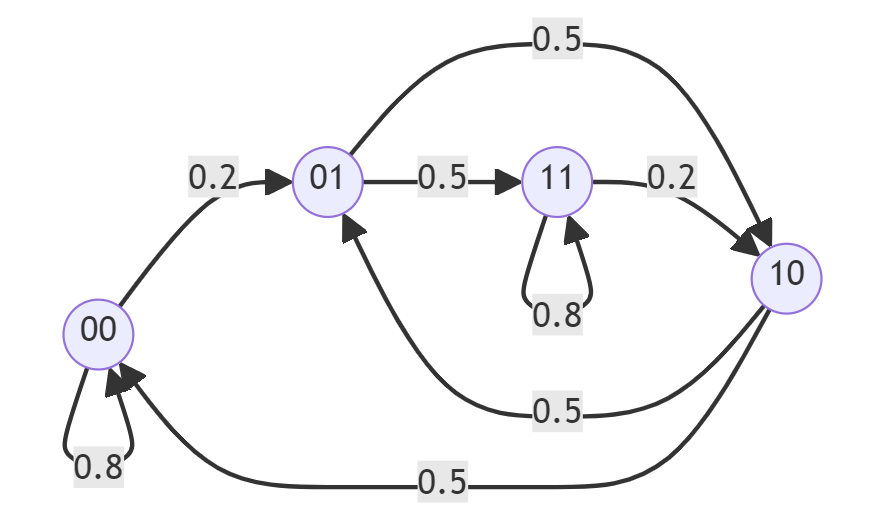
\includegraphics[width=0.5\textwidth]{./entropia_y_fuentes/img/mermaid1.png}
\end{figure}

\textbf{
Calcula las probabilidades de los estados en estado estacionario y la entropía de la fuente.
}

\vspace{0.5cm}

De la imagen tenemos las probabilidades condicionales:

\begin{align*}
    P(0|00) &= 0.8\\
    P(1|00) &= 0.2\\
    P(0|01) &= 0.5\\
    P(1|01) &= 0.5\\
    P(0|10) &= 0.5\\
    P(1|10) &= 0.5\\
    P(0|11) &= 0.2\\
    P(1|11) &= 0.8
\end{align*}

esto nos permite calcular las probabilidades de los estados en estado estacionario mediante un sistema de ecuaciones:

\begin{align*}
    &\begin{cases}
    P(00) &= P(00)P(0|00) + P(10)P(0|10)\\
    P(01) &= P(00)P(1|00) + P(10)P(1|10)\\
    P(10) &= P(01)P(0|01) + P(11)P(0|11)\\
    1 &= P(00) + P(01) + P(10) + P(11)
    \end{cases}\\
    &\begin{cases}
    P(00) &= P(00)0.8 + P(10)0.5\\
    P(01) &= P(00)0.2 + P(10)0.5\\
    P(10) &= P(01)0.5 + P(11)0.2\\
    1 &= P(00) + P(01) + P(10) + P(11)
    \end{cases}\\
    &\begin{cases}
    0 &= - P(00)0.2 + P(10)0.5\\
    0 &= P(00)0.2 - P(01) + P(10)0.5\\
    0 &= P(01)0.5 - P(10) + P(11)0.2\\
    1 &= P(00) + P(01) + P(10) + P(11)
    \end{cases}\Rightarrow P(00) = \frac{5}{2}P(10)\\
    &\begin{cases}
    0 &= - P(01) + P(10)\\
    0 &= P(01)0.5 - P(10) + P(11)0.2\\
    1 &= P(01) + \frac{7}{2}P(10) + P(11)
    \end{cases}\Rightarrow P(01) = P(10)\\
    &\begin{cases}
        0 &= - 0.5P(10) + P(11)0.2\\
        1 &= \frac{9}{2}P(10) + P(11)
    \end{cases}\Rightarrow P(11) = \frac{5}{2}P(10)\\
    &\begin{cases}
        1 &= 7P(10)
    \end{cases}\Rightarrow P(10) = \frac{1}{7}\approx 0.14\\
    &\begin{cases}
        P(00) &= \frac{5}{2}P(10) = \frac{5}{14}\approx 0.36\\
        P(01) &= P(10) = \frac{1}{7}\approx 0.14\\
        P(11) &= \frac{5}{2}P(10) = \frac{5}{14}\approx 0.36\\
    \end{cases}
\end{align*}

La entropia de la fuente es:

\begin{align*}
    H(X) &= -\sum_{i=1}^{4}\sum_{j=1}^{4}P(x_i)P(y_j|x_i)\log\left(P(y_j|x_i)\right)\\
    &= -P(00)P(0|00)\log\left(P(0|00)\right) - P(00)P(1|00)\log\left(P(1|00)\right)\\
    &- P(01)P(0|01)\log\left(P(0|01)\right) - P(01)P(1|01)\log\left(P(1|01)\right)\\
    &- P(10)P(0|10)\log\left(P(0|10)\right) - P(10)P(1|10)\log\left(P(1|10)\right)\\
    &- P(11)P(0|11)\log\left(P(0|11)\right) - P(11)P(1|11)\log\left(P(1|11)\right)\\
    &\approx 0.79
\end{align*}

\pagebreak

\textbf{
10. Sea una fuente de Markov de primer orden sobre el alfabeto $\mathcal{S}=\left\{a,b,c\right\}$ definida por el siguiente diagrama de estados:
}

\begin{figure}[htbp!]
    \centering
    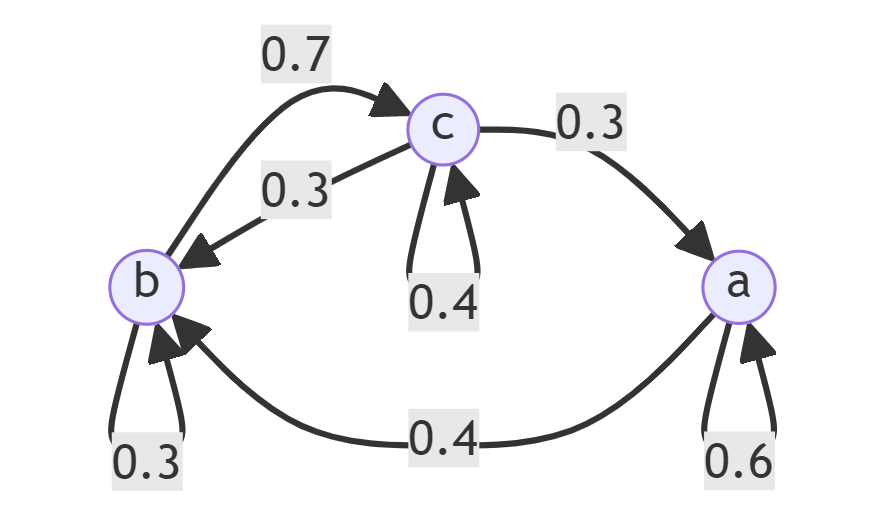
\includegraphics[width=0.5\textwidth]{./entropia_y_fuentes/img/mermaid2.png}
\end{figure}

\textbf{Calcula:}

\begin{itemize}
    \item\textbf{La probabilidad de cada estado en régimen estacionario.}
    \item\textbf{La entropía de la fuente.}
    \item\textbf{La fuente afín.}
    \item\textbf{La entropía de La fuente afín.}
\end{itemize}

\vspace{0.5cm}

De la imagen tenemos las probabilidades condicionales:

\begin{align*}
    P(a|a) &= 0.6\\
    P(b|a) &= 0.4\\
    P(b|b) &= 0.3\\
    P(c|b) &= 0.7\\
    P(a|c) &= 0.3\\
    P(b|c) &= 0.3\\
    P(c|c) &= 0.4
\end{align*}

Esto nos permite calcular las probabilidades de los estados en estado estacionario mediante un sistema de ecuaciones:

\begin{align}
    &\begin{cases}
    P(a) &= P(a)P(a|a) + P(c)P(a|c)\\
    P(b) &= P(a)P(b|a) + P(b)P(b|b) + P(c)P(b|c)\\
    1 &= P(a) + P(b) + P(c)
    \end{cases}\\
    &\begin{cases}
    P(a) &= P(a)0.6 + P(c)0.3\\
    P(b) &= P(a)0.4 + P(b)0.3 + P(c)0.3\\
    1 &= P(a) + P(b) + P(c)
    \end{cases}\\
    &\begin{cases}
    0 &= -0.4P(a) + 0.3P(c)\\
    0 &= 0.4P(a) - 0.7P(b) + 0.3P(c)\\
    1 &= P(a) + P(b) + P(c)
    \end{cases} \Rightarrow P(a) = \frac{3}{4}P(c)\\
    &\begin{cases}
    0 &= - 0.7P(b) + 0.6P(c)\\
    1 &= \frac{7}{4}P(c) + P(b)
    \end{cases} \Rightarrow P(b) = \frac{6}{7}P(c)\\
    &\begin{cases}
    1 &= \frac{73}{28}P(c) 
    \end{cases} \Rightarrow P(c) = \frac{28}{73}\\
    &\begin{cases}
    P(a) &= \frac{21}{73}\\
    P(b) &= \frac{24}{73}\\
    P(c) &= \frac{28}{73}
    \end{cases}
\end{align}

La entropía de la fuente es:

\begin{align*}
    H(S) &= -\sum_{i=1}^{3}\sum_{j=1}^{3}P(x_i)P(y_j|x_i)\log\left(P(y_j|x_i)\right)\\
    &= -P(a)P(a|a)\log\left(P(a|a)\right) - P(a)P(b|a)\log\left(P(b|a)\right)\\
    &- P(b)P(b|b)\log\left(P(b|b)\right) - P(b)P(c|b)\log\left(P(c|b)\right)\\
    &- P(c)P(a|c)\log\left(P(a|c)\right) - P(c)P(b|c)\log\left(P(b|c)\right) - P(c)P(c|c)\log\left(P(c|c)\right)\\
    &\approx 1.17
\end{align*}

Como se trata de una fuente de Markov de primer orden, la fuente afín es se define como el alfabeto $\mathcal{A}=\left\{a,b,c\right\}$ con las probabilidades $P(a) = \frac{21}{73}$, $P(b) = \frac{24}{73}$ y $P(c) = \frac{28}{73}$. La entropía de la fuente afín es:

\begin{align*}
    H(S) &= -\sum_{i=1}^{3}P(x_i)\log\left(P(x_i)\right)\\
    &= -\frac{21}{73}\log\left(\frac{21}{73}\right) - \frac{24}{73}\log\left(\frac{24}{73}\right) - \frac{28}{73}\log\left(\frac{28}{73}\right)\\
    &\approx 1.57
\end{align*}

\section{Ejercicios de Códigos}

\textbf{
1. Sea la codificación bloque $f:\mathcal{A}^+\rightarrow\mathcal{B}^+$ en la que $\mathcal{A}=\left\{a,b,c\right\}$, $\mathcal{B}=\left\{0,1\right\}$ y $f(a)=0$, $f(b) = 01$, $f(c)=11$. ¿Es $f$ unívocamente decodificable?
}

\vspace{0.5cm}

El primer paso del algoritmo consiste en comprobar si la codificación es singular. Vemos que no es singular ya que no hay dos elementos en $f\left(\mathcal{A}\right)=\left\{0,01,11\right\}$ que sean iguales.

El siguiente paso consiste en definirnos el conjunto $A$, que es el conjunto de todos los sufijos que hemos de añadir a los códigos de $f\left(\mathcal{A}\right)$ para que sean prefijos de otros códigos. En este caso, $A=\left\{1\right\}$.

A continuación calculamos la intersección entre $f\left(\mathcal{A}\right)$ y $A$; si esta intersección no es vacía, la codificación no es unívocamente decodificable. En este caso, $f\left(\mathcal{A}\right)\cap A = \emptyset$.

Procedemos con el siguiente paso. Definimos el conjunto $A'=\emptyset$. Mientras $A$ no sea vacío, repetimos los siguientes pasos:

\begin{enumerate}
    \item Re-definimos $A'$ como $A'\cup A$. En este caso, $A'=\left\{1\right\}$.
    \item Nos definimos el conjunto $B$ como el conjunto que contiene todos los sufijos de tal forma que concatenados a algún código, obtenemos un elemento de $A$; además también añadimos a este conjunto los sufijos tales que concatenados a algún elemento de $A$, obtenemos un código. En este caso $B=\left\{1\right\}$.
    \item Ahora nos re-definimos el conjunto $A$ como $B-A'$. En este caso, $A=\emptyset$.
    \item Computamos ahora $A\cap f\left(\mathcal{A}\right)$. Si este conjunto no es vacío, la codificación no es unívocamente decodificable. En este caso, $A\cap f\left(\mathcal{A}\right)=\emptyset$.
    \item Ahora tenemos que mirar si podemos volver a entrar en el bucle while.
\end{enumerate}

Como terminamos la iteración con $A=\emptyset$, salimos del bucle y sabemos que la codificación es unívocamente decodificable.

\vspace{1cm}

\textbf{
2. Sea la codificación bloque $f:\mathcal{A}^+\rightarrow\mathcal{B}^+$ en la que $\mathcal{A}=\left\{a,b,c,d\right\}$, $\mathcal{B}=\left\{a,b\right\}$ y $f(a)=ab$, $f(b) = aaab$, $f(c)=aba$, $f(d)=aab$. ¿Es $f$ unívocamente decodificable?
}

\vspace{0.5cm}

Los próximos ejercicios de este tipo los haré de forma más resumida, ya que el procedimiento es el mismo que en el ejercicio anterior.

\begin{itemize}
    \item $f\left(\mathcal{A}\right)=\left\{ab,aaab,aba,aab\right\}$, no es singular.
    \item $A=\left\{a\right\}$
    \item $f\left(\mathcal{A}\right)\cap A = \emptyset$
    \item $A'=\emptyset$
    \item $A'=\left\{a\right\}$
    \item $B = \left\{b, aab, ba, ab\right\}$
    \item $A = B-A' = \left\{b, aab, ba, ab\right\}$
    \item $A\cap f\left(\mathcal{A}\right) = \left\{ab, aab\right\}\neq\emptyset$, por lo tanto no es unívocamente decodificable.
\end{itemize}

\vspace{1cm}

\textbf{
3. Sea la codificación bloque $f:\mathcal{A}^+\rightarrow\mathcal{B}^+$ en la que $\mathcal{A}=\left\{a,b,c,d\right\}$, $\mathcal{B}=\left\{a,b\right\}$ y $f(a)=aba$, $f(b) = a$, $f(c)=bab$, $f(d)=bb$. ¿Es $f$ unívocamente decodificable?
}

\vspace{0.5cm}

\begin{itemize}
    \item $f\left(\mathcal{A}\right)=\left\{aba,a,bab,bb\right\}$, no es singular.
    \item $A = \left\{ba\right\}$
    \item $f\left(\mathcal{A}\right)\cap A = \emptyset$
    \item $A'=\emptyset$
    \item $A'=\left\{ba\right\}$
    \item $B = \left\{b\right\}$
    \item $A = B-A' = \left\{b\right\}$
    \item $A\cap f\left(\mathcal{A}\right) = \emptyset$
    \item $A'=\left\{ba,b\right\}$
    \item $B=\left\{ab, b\right\}$
    \item $A = B-A' = \left\{ab\right\}$
    \item $A\cap f\left(\mathcal{A}\right) = \emptyset$
    \item $A'=\left\{ba,b,ab\right\}$
    \item $B = \left\{b, a\right\}$
    \item $A = \left\{a\right\}$
    \item $A\cap f\left(\mathcal{A}\right) =\left\{a\right\}\neq \emptyset$, por lo tanto no es unívocamente decodificable.
\end{itemize}

\vspace{1cm}

\textbf{
4. Sea la codificación bloque $f:\mathcal{A}^+\rightarrow\mathcal{B}^+$ en la que $\mathcal{A}=\left\{a,b,c,d\right\}$, $\mathcal{B}=\left\{a,b\right\}$ y $f(a)=a$, $f(b) = abb$, $f(c)=aba$, $f(d)=bab$. ¿Es $f$ unívocamente decodificable?
}

\vspace{0.5cm}

\begin{itemize}
    \item $f\left(\mathcal{A}\right)=\left\{a,abb,aba,bab\right\}$, no es singular.
    \item $A=\left\{ba, bb\right\}$
    \item $f\left(\mathcal{A}\right)\cap A = \emptyset$
    \item $A'=\emptyset$
    \item $A'=\left\{ba, bb\right\}$
    \item $B = \left\{b\right\}$
    \item $A = B-A' = \left\{b\right\}$
    \item $A\cap f\left(\mathcal{A}\right) = \emptyset$
    \item $A'=\left\{ba, bb, b\right\}$
    \item $B = \left\{ab\right\}$
    \item $A = B-A' = \left\{ab\right\}$
    \item $A\cap f\left(\mathcal{A}\right) = \emptyset$
    \item $A'=\left\{ba, bb, b, ab\right\}$
    \item $B = \left\{b, a\right\}$
    \item $A = B - A' = \left\{a\right\}$
    \item $A\cap f\left(\mathcal{A}\right) \neq\emptyset$ por lo tanto no es unívocamente decodificable.
\end{itemize}

\vspace{1cm}

\textbf{
5. Sea la codificación bloque $f:\mathcal{A}^+\rightarrow\mathcal{B}^+$ en la que $\mathcal{A}=\left\{a,b,c,d\right\}$, $\mathcal{B}=\left\{a,b\right\}$ y $f(a)=aba$, $f(b) = ab$, $f(c)=abb$, $f(d)=bbcb$. ¿Es $f$ unívocamente decodificable?
}

\vspace{0.5cm}

\begin{itemize}
    \item $f\left(\mathcal{A}\right)=\left\{aba,ab,abb,bbcb\right\}$, no es singular.
    \item $A=\left\{a, b\right\}$
    \item $f\left(\mathcal{A}\right)\cap A = \emptyset$
    \item $A'=\emptyset$
    \item $A'=\left\{a, b\right\}$
    \item $B = \left\{ba, b, bb, bcb\right\}$
    \item $A = B-A' = \left\{ba, bb, bcb\right\}$
    \item $A\cap f\left(\mathcal{A}\right) = \emptyset$
    \item $A'=\left\{a, b, ba, bb, bcb\right\}$
    \item $B = \left\{cb\right\}$
    \item $A = B-A' = \left\{cb\right\}$
    \item $A\cap f\left(\mathcal{A}\right) = \emptyset$
    \item $A'=\left\{a, b, ba, bb, bcb, cb\right\}$
    \item $B = \emptyset$
    \item $A = B-A' = \emptyset$
    \item $A\cap f\left(\mathcal{A}\right) = \emptyset$
    \item Como $A$ es vacío, la codificación es unívocamente decodificable.
\end{itemize}

\vspace{1cm}

\textbf{
6. Sea la codificación bloque $f:\mathcal{A}^+\rightarrow\mathcal{B}^+$ en la que $\mathcal{A}=\left\{a,b,c,d,e\right\}$, $\mathcal{B}=\left\{0,1\right\}$ y $\left|f(a)\right|=4$, $\left|f(b)\right|=4$, $\left|f(c)\right|=1$, $\left|f(d)\right|=2$, $\left|f(e)\right|=3$.
}

\begin{itemize}
    \item\textbf{Demuestra que cumple la igualdad de Kraft}.
    \item\textbf{Particulariza $f$ para que $f\left(\mathcal{A}\right)$ sea un código completo alfabéticamente ajustado a la ordenación generada por $0<1$}.
\end{itemize}

\vspace{0.5cm}

Para demostrar que cumple la igualdad de Kraft, tomamos $k=\left|\mathcal{B}\right|=2$ y calculamos:

\begin{align*}
    \sum_{i=1}^{5}2^{-\left|f(a_i)\right|} &= 2^{-4} + 2^{-4} + 2^{-1} + 2^{-2} + 2^{-3}\\
    &= \frac{1}{16} + \frac{1}{16} + \frac{1}{2} + \frac{1}{4} + \frac{1}{8}\\
    &= 1
\end{align*}

Una particularización (en la que no conservamos el orden del alfabeto fuente), podría ser:

\begin{align*}
    f(a) &= 1110\\
    f(b) &= 1111\\
    f(c) &= 0\\
    f(d) &= 10\\
    f(e) &= 110
\end{align*}

\vspace{1cm}

\textbf{
7. Sea la codificación bloque $f:\mathcal{A}^+\rightarrow\mathcal{B}^+$ en la que $\mathcal{A}=\left\{a_1,a_2,a_3,a_4,a_5,a_6,a_7\right\}$, $\mathcal{B}=\left\{a,b,c\right\}$ con $\left|f(a_1)\right|=3$, $\left|f(a_2)\right|=2$, $\left|f(a_3)\right|=2$, $\left|f(a_4)\right|=3$, $\left|f(a_5)\right|=1$, $\left|f(a_6)\right|=3$, $\left|f(a_7)\right|=1$. ¿Cumple $f$ con la desigualdad de Kraft? Define $f$, si es posible, de modo que ea una codificación bloque instantánea alfabéticamente ordenada. ¿Es completa?
}

\vspace{0.5cm}

Para comprobar si cumple la desigualdad de Kraft, calculamos:

\begin{align*}
    \sum_{i=1}^{7}2^{-\left|f(a_i)\right|} &= 3^{-3} + 3^{-2} + 3^{-2} + 3^{-3} + 3^{-1} + 3^{-3} + 3^{-1}\\
    &= \frac{1}{27} + \frac{1}{9} + \frac{1}{9} + \frac{1}{27} + \frac{1}{3} + \frac{1}{27} + \frac{1}{3}\\
    &= 1
\end{align*}

Una posible codificación bloque instantánea alfabéticamente ordenada sería:

\begin{align*}
    f(a_1) &= cca\\
    f(a_2) &= ca\\
    f(a_3) &= cb\\
    f(a_4) &= ccb\\
    f(a_5) &= a\\
    f(a_6) &= ccc\\
    f(a_7) &= b
\end{align*}

La codificación es completa.

\pagebreak

\textbf{
8. Sea una fuente de memoria nula $FI=\left(\mathcal{A},p\right)$ con $\mathcal{A}=\left\{a_1,a_2,a_3,a_4\right\}$ y probabilidades $p(a_1)=0.4$, $p(a_2)=0.3$, $p(a_3)=0.2$, $p(a_4)=0.1$. Obtén una codificación bloque instantánea $f$ con el alfabéto código $\left\{0,1\right\}$ para la fuente de información.
}

\vspace{0.5cm}

Utilizando el método de Shannon:

\begin{table}[htbp!]
    \centering
    \begin{tabular}{|l|l|l|l|l|}
    \hline
    Símbolo & $p$ & $-\log\left(p\right)$ & $l$ & código \\
    \hline
    $a_1$ & 0.4 & 1.32 & 2 & 00 \\
    $a_2$ & 0.3 & 1.73 & 2 & 01 \\
    $a_3$ & 0.2 & 2.32 & 3 & 100 \\
    $a_4$ & 0.1 & 3.32 & 4 & 1010 \\
    \hline
    \end{tabular}    
\end{table}

\vspace{1cm}

\textbf{
9. Sea una fuente de memoria nula $FI=\left(\mathcal{A},p\right)$ con $\mathcal{A}=\left\{a_1,a_2,a_3,a_4,a_5,a_6\right\}$ y probabilidades $p(a_1)=0.1$, $p(a_2)=0.1$, $p(a_3)=0.2$, $p(a_4)=0.2$, $p(a_5)=0.3$ y $p(a_6)=0.1$. Obtén una codificación bloque instantánea $f$ con el alfabéto código $\left\{0,1\right\}$ para la fuente de información.
}

\vspace{0.5cm}

Utilizando el método de Shannon:	

\begin{table}[htbp!]
    \centering
    \begin{tabular}{|l|l|l|l|l|}
    \hline
    Símbolo & $p$ & $-\log\left(p\right)$ & $l$ & código \\
    \hline
    $a_1$ & 0.1 & 3.32 & 4 & 1000 \\
    $a_2$ & 0.1 & 3.32 & 4 & 1001 \\
    $a_3$ & 0.2 & 2.32 & 3 & 010 \\
    $a_4$ & 0.2 & 2.32 & 3 & 011 \\
    $a_5$ & 0.3 & 1.73 & 2 & 00 \\
    $a_6$ & 0.1 & 3.32 & 4 & 1010 \\
    \hline
    \end{tabular}
\end{table}
\end{document}